\chapter{Enoles, enolatos y reacción aldólica}\label{ch:b2:enolates-aldol}

Cada vez que una célula degrada la glucosa, una enzima corta un fosfato de azúcar de seis carbonos
en dos fragmentos de tres carbonos: una reacción \omterm{def:b2:enolates-aldol:aldol}{aldólica} en sentido inverso. En sentido
directo, la misma reacción une dos compuestos carbonílicos en uno solo, y es
el método más usado por los químicos para formar enlaces carbono--carbono. Se basa en una
propiedad que los capítulos anteriores solo rozaron: los átomos de hidrógeno contiguos a un
grupo carbonilo son ácidos, y arrancar uno convierte el carbono vecino del
carbonilo en un nucleófilo.

\begin{recall}
El volumen del primer año: $\mathrm pK_a$ y reacción prioritaria, carbaniones, control cinético y
termodinámico, adiciones nucleófilas a los carbonilos, eliminaciones E1 y E2, hidratación de los
alquinos (un \omterm{def:b2:enolates-aldol:tautomerism}{enol} que se reorganiza). \Cref{ch:b2:frontier-orbitals}: \omterm{def:b2:frontier-orbitals:ambident}{nucleófilos ambidentados}.
\Cref{ch:b2:acyl-substitution}: ésteres y sustitución de acilo.
\end{recall}

\section{Tautomería ceto--enólica}

\begin{definition}[Tautomería]\label{def:b2:enolates-aldol:tautomerism}
Los \emph{tautómeros}\index{tautomeros@tautómeros} son isómeros que se interconvierten por desplazamiento de un hidrógeno y de un doble
enlace. En la \emph{tautomería ceto--enólica}\index{tautomeria ceto--enolica@tautomería ceto--enólica}, un compuesto carbonílico con un
hidrógeno en el carbono contiguo al carbonilo (la forma ceto) está en equilibrio con su
\emph{enol}\index{enol}, un alcohol situado sobre un doble enlace \ce{C=C}.
\end{definition}

\begin{omfigure}
\setchemfig{atom sep=2em}
\schemestart
\chemfig{H_3C-C(=[2]O)-CH_3}
\arrow{<=>[\ce{H+} o \ce{HO-}][catálisis]}[,2.2]
\chemfig{H_3C-C(-[2]OH)=CH_2}
\schemestop
\par\vspace{6pt}

{\small La propanona y su \omterm{def:b2:enolates-aldol:tautomerism}{enol}, el prop-1-en-2-ol. Un ácido (protonación del oxígeno carbonílico y luego pérdida
de un hidrógeno $\alpha$) o una base (arranque de un hidrógeno $\alpha$ y luego protonación del oxígeno)
catalizan la interconversión; el equilibrio está muy desplazado hacia la forma ceto.}
\end{omfigure}

\begin{proposition}[Contenido en enol]\label{prop:b2:enolates-aldol:enol-content}
Los aldehídos y cetonas sencillos contienen solo trazas de \omterm{def:b2:enolates-aldol:tautomerism}{enol}; los compuestos 1,3-dicarbonílicos como
la pentano-2,4-diona contienen una gran proporción de él.
\end{proposition}

\begin{proof}[Argumento]
Un enlace \ce{C=O} es más fuerte que un enlace \ce{C=C} en mayor medida de lo que un enlace \ce{O-H} es más débil que un enlace
\ce{C-H}: la forma ceto está favorecida. En un compuesto 1,3-dicarbonílico, el doble enlace del \omterm{def:b2:enolates-aldol:tautomerism}{enol} está conjugado
con el segundo grupo carbonilo, y el \ce{OH} del \omterm{def:b2:enolates-aldol:tautomerism}{enol} forma un enlace de hidrógeno interno con su oxígeno
en un anillo de seis eslabones: ambos efectos estabilizan el \omterm{def:b2:enolates-aldol:tautomerism}{enol} lo suficiente para que sea una forma mayoritaria.
\end{proof}

Como el \omterm{def:b2:enolates-aldol:tautomerism}{enol} es plano en su \ce{C=C}, un estereocentro en el carbono $\alpha$ se pierde cada vez que
se forma el \omterm{def:b2:enolates-aldol:tautomerism}{enol}: una cetona ópticamente activa con un estereocentro contiguo a su carbonilo se racemiza en medio ácido
o básico.

\section{Enolatos}

\begin{definition}[Enolatos]\label{def:b2:enolates-aldol:enolate}
El \emph{carbono $\alpha$}\index{carbono alfa@carbono $\alpha$} de un compuesto carbonílico es el carbono
unido al carbono carbonílico; sus hidrógenos son los \emph{hidrógenos $\alpha$}\index{hidrogeno alfa@hidrógeno $\alpha$}.
Arrancar uno da un \emph{ion enolato}\index{ion enolato}, cuya
carga negativa se reparte entre el carbono $\alpha$ y el oxígeno.
\end{definition}

\begin{proposition}[Acidez de los hidrógenos $\alpha$]\label{prop:b2:enolates-aldol:alpha-acidity}
Los hidrógenos $\alpha$ son mucho más ácidos que los enlaces \ce{C-H} ordinarios porque el \omterm{def:b2:enolates-aldol:enolate}{enolato} está estabilizado
por resonancia; un hidrógeno situado entre dos grupos carbonilo es lo bastante ácido para que lo arranque un alcóxido o
incluso el hidróxido.
\end{proposition}

\begin{proof}[Argumento]
En el \omterm{def:b2:enolates-aldol:enolate}{enolato} la carga negativa reside en parte sobre el oxígeno, electronegativo; un segundo carbonilo al
otro lado la deslocaliza sobre dos oxígenos. Medidos en agua, la pentano-2,4-diona tiene $\mathrm pK_a =
9.0$ y el 3-oxobutanoato de etilo 10.7, comparables con el nitrometano (10.2), cuyo anión está estabilizado
por el grupo nitro del mismo modo; una cetona sencilla, con un solo carbonilo, es mucho más débil, demasiado débil
para que su acidez pueda medirse directamente en agua.
% ledger: pka:acac, pka:acetoacetate, pka:nitromethane
\end{proof}

\begin{omfigure}
\setchemfig{atom sep=2em}
\schemestart
\chemfig{H_3C-C(=[2]O)-\chemabove{C}{\scriptstyle -}H_2}
\arrow{<->}
\chemfig{H_3C-C(-[2]\chemabove{O}{\scriptstyle -})=CH_2}
\schemestop
\par\vspace{6pt}

{\small Las dos estructuras de resonancia del \omterm{def:b2:enolates-aldol:enolate}{enolato} de la propanona. La carga negativa se reparte entre
el carbono $\alpha$ y el oxígeno: el \omterm{def:b2:enolates-aldol:enolate}{enolato} es un \omterm{def:b2:frontier-orbitals:ambident}{nucleófilo ambidentado}, que reacciona con la mayoría de los electrófilos
carbonados por el carbono.}
\end{omfigure}

\begin{definition}[Enolatos cinético y termodinámico]\label{def:b2:enolates-aldol:kinetic-enolate}
Para una cetona con dos carbonos $\alpha$ distintos, el \emph{enolato cinético}\index{enolato cinetico@enolato cinético}
es el que se forma más deprisa, por arranque de un hidrógeno del lado menos impedido y menos sustituido; el
\emph{enolato termodinámico}\index{enolato termodinamico@enolato termodinámico} es el más estable, con el doble enlace más
sustituido.
\end{definition}

\begin{proposition}[Elegir el enolato]\label{prop:b2:enolates-aldol:enolate-control}
Una base fuerte y voluminosa usada en cantidad completa a baja temperatura (diisopropilamiduro de litio, LDA, a
\qty{-78}{\degreeCelsius}) forma el \omterm{def:b2:enolates-aldol:kinetic-enolate}{enolato cinético} de forma completa e irreversible; una base más débil a temperatura
ambiente (un alcóxido en su alcohol) deja que los \omterm{def:b2:enolates-aldol:enolate}{enolatos} se interconviertan y da sobre todo el
termodinámico.
\end{proposition}

\begin{proof}[Argumento]
El LDA ($\mathrm pK_a$ de la diisopropilamina cercano a 36, muy por encima del de la cetona) desprotona por completo y
deprisa; a baja temperatura el \omterm{def:b2:enolates-aldol:enolate}{enolato} no se reprotona, y decide la desprotonación más rápida, en el
\ce{CH2} o el \ce{CH3} accesible: control cinético. Un alcóxido arranca el protón solo en parte,
los \omterm{def:b2:enolates-aldol:enolate}{enolatos} y la cetona intercambian protones continuamente, y la mezcla en equilibrio favorece el
\omterm{def:b2:enolates-aldol:enolate}{enolato} más sustituido, más estable: control termodinámico (como en el volumen del primer año).
% ledger: ghs:LDA
\end{proof}

\section{Alquilación de los enolatos}

Los \omterm{def:b2:enolates-aldol:enolate}{enolatos} atacan a los halogenoalcanos primarios por sustitución bimolecular, formando un nuevo enlace \ce{C-C} en
el carbono $\alpha$. Con los hidrógenos $\alpha$ muy ácidos de un compuesto 1,3-dicarbonílico basta un alcóxido,
y el carbonilo adicional puede eliminarse después.

\begin{definition}[Descarboxilación]\label{def:b2:enolates-aldol:decarboxylation}
Una \emph{descarboxilación}\index{descarboxilacion@descarboxilación} elimina un grupo carboxilo en forma de \ce{CO2}. En la
\emph{síntesis malónica}\index{sintesis malonica@síntesis malónica}, el propanodioato de dietilo se desprotona,
se alquila, se hidroliza al ácido propanodioico sustituido y se descarboxila por calentamiento, lo que da un
ácido carboxílico \ce{RCH2COOH}.
\end{definition}

\begin{proposition}[Descarboxilaciones fáciles]\label{prop:b2:enolates-aldol:decarboxylation}
Los $\beta$-cetoácidos y los ácidos propanodioicos pierden \ce{CO2} por calentamiento suave; los ácidos carboxílicos ordinarios
no.
\end{proposition}

\begin{proof}[Argumento]
El carbonilo situado a dos enlaces del grupo carboxilo acepta el hidrógeno del \ce{COOH} en un estado de transición
cíclico de seis eslabones mientras sale el \ce{CO2}: se forma directamente un \omterm{def:b2:enolates-aldol:tautomerism}{enol}, que luego tautomeriza. Sin
ese carbonilo, el carbanión que dejaría la pérdida de \ce{CO2} no tendría ninguna estabilización.
\end{proof}

\begin{definition}[Reacción del haloformo]\label{def:b2:enolates-aldol:haloform}
La \emph{reacción del haloformo}\index{reaccion del haloformo@reacción del haloformo} convierte una metilcetona \ce{RCOCH3}, con un
halógeno y un exceso de hidróxido, en un carboxilato \ce{RCOO-} y un haloformo \ce{CHX3}.
\end{definition}

Cada halógeno introducido hace más ácidos los hidrógenos $\alpha$ restantes, de modo que el grupo metilo
se trihalogena; el grupo \ce{CX3-} es entonces un grupo saliente lo bastante bueno para que el hidróxido lo expulse en una
sustitución de acilo. Con yodo, el precipitado amarillo de yodoformo es un ensayo de las metilcetonas.

\section{La reacción aldólica}

\begin{definition}[Reacciones aldólicas]\label{def:b2:enolates-aldol:aldol}
En una \emph{adición aldólica}\index{adicion aldolica@adición aldólica} el \omterm{def:b2:enolates-aldol:enolate}{enolato} (o el \omterm{def:b2:enolates-aldol:tautomerism}{enol}) de un compuesto carbonílico se adiciona
al grupo carbonilo de otro, dando un compuesto $\beta$-hidroxicarbonílico, un
\emph{aldol}\index{aldol}. En una \emph{condensación aldólica}\index{condensacion aldolica@condensación aldólica} el aldol pierde
agua, dando un compuesto carbonílico $\alpha,\beta$-insaturado (una enona o un enal).
\end{definition}

\begin{omfigure}
\setchemfig{atom sep=1.9em}
\schemestart
\chemfig{H_3C-CH=O} \+ \chemfig{^{-}CH_2-CH=O}
\arrow{->[adición]}
\chemfig{H_3C-CH(-[2]O^{-})-CH_2-CH=O}
\schemestop

\medskip
\schemestart
\arrow{->[\ce{H2O}][$-$ \ce{HO-}]}
\chemfig{H_3C-CH(-[2]OH)-CH_2-CH=O}
\arrow{->[calor, base][$-$ \ce{H2O}]}
\chemfig{H_3C-CH=CH-CH=O}
\schemestop
\par\vspace{6pt}

{\small La reacción \omterm{def:b2:enolates-aldol:aldol}{aldólica} del etanal. El \omterm{def:b2:enolates-aldol:enolate}{enolato} se adiciona a una segunda molécula de etanal; la protonación
da el \omterm{def:b2:enolates-aldol:aldol}{aldol}, el 3-hidroxibutanal. Al calentar con base, se arranca un hidrógeno $\alpha$ y el hidróxido
sale del carbono $\beta$: but-2-enal, conjugado.}
\end{omfigure}

\begin{proposition}[Desplazar la reacción aldólica]\label{prop:b2:enolates-aldol:aldol-equilibrium}
La \omterm{def:b2:enolates-aldol:aldol}{adición aldólica} es reversible; la deshidratación, que forma un sistema conjugado, arrastra la
reacción hacia el producto de condensación.
\end{proposition}

\begin{proof}[Argumento]
Dos moléculas dan una, de modo que la \omterm{def:b2:reaction-free-energy:reaction-entropy}{entropía de reacción} es negativa, y el nuevo enlace \ce{C-C} apenas
compensa el enlace $\pi$ \ce{C=O} perdido: para muchas cetonas $K$ es pequeña. Retirar el \omterm{def:b2:enolates-aldol:aldol}{aldol} por deshidratación
mantiene $Q < K$ para la adición; la enona conjugada formada está estabilizada y, a alta temperatura,
la ganancia de entropía al liberar agua la favorece aún más. La reacción inversa, la retroaldólica, es la
etapa por la que la célula escinde un azúcar de seis carbonos.
\end{proof}

\begin{method}[Controlar una aldólica cruzada]\label{met:b2:enolates-aldol:crossed-aldol}
\begin{enumerate}
  \item Úsese un compañero sin hidrógenos $\alpha$ (benzaldehído, metanal): solo puede ser el
        electrófilo.
  \item O bien fórmese primero por completo el \omterm{def:b2:enolates-aldol:enolate}{enolato} de uno de los compañeros (LDA, \qty{-78}{\degreeCelsius}), y añádase luego
        el otro.
  \item O bien úsese un compañero 1,3-dicarbonílico, mucho más ácido que el otro.
  \item Prefiérase un aldehído como electrófilo: es más reactivo que una cetona.
\end{enumerate}
\end{method}

\begin{method}[Reconocer un producto aldólico]\label{met:b2:enolates-aldol:aldol-recognition}
\begin{enumerate}
  \item Búsquese un \ce{C=O} con un \ce{OH} en el carbono situado a dos átomos ($\beta$), o un \ce{C=C}
        conjugado con un \ce{C=O}.
  \item Córtese el enlace entre los carbonos $\alpha$ y $\beta$: el carbono $\beta$ era un carbono carbonílico (el
        electrófilo), y el carbono $\alpha$, el carbono del \omterm{def:b2:enolates-aldol:enolate}{enolato}.
  \item Compruébese que los dos compañeros existen y que el \omterm{def:b2:enolates-aldol:enolate}{enolato} puede formarse selectivamente.
\end{enumerate}
\end{method}

\section{La condensación de Claisen}

\begin{definition}[Condensación de Claisen]\label{def:b2:enolates-aldol:claisen}
En una \emph{condensación de Claisen}\index{condensacion de Claisen@condensación de Claisen}, el \omterm{def:b2:enolates-aldol:enolate}{enolato} de un éster ataca el
carbonilo de otra molécula de éster en una sustitución de acilo, dando un \emph{$\beta$-cetoéster}\index{beta-cetoester@$\beta$-cetoéster}
y liberando un alcóxido. Su versión intramolecular, la ciclación de
Dieckmann, da un $\beta$-cetoéster cíclico.
\end{definition}

\begin{proposition}[Qué impulsa la condensación de Claisen]\label{prop:b2:enolates-aldol:claisen-drive}
La \omterm{def:b2:enolates-aldol:claisen}{condensación de Claisen} del etanoato de etilo necesita un equivalente completo de etóxido de sodio: su equilibrio
es desfavorable, y lo impulsa la desprotonación del $\beta$-cetoéster formado.
\end{proposition}

\begin{proof}
La condensación propiamente dicha, \ce{2CH3COOEt <=> CH3COCH2COOEt + EtOH}, tiene una constante de equilibrio
$K_1$ pequeña. El $\beta$-cetoéster ($\mathrm pK_a = 10.7$) se desprotona después por el etóxido (etanol, 15.9):
$K_2 = 10^{15.9 - 10.7} = 10^{5.2}$. La reacción global, condensación más desprotonación, tiene
$K_1K_2$, suficientemente grande incluso para $K_1$ pequeña; la base se consume y un tratamiento ácido da el
$\beta$-cetoéster neutro. Un éster con un solo hidrógeno $\alpha$, cuyo producto no puede desprotonarse, da
poco producto.
% ledger: pka:acetoacetate, pka:ethanol
\end{proof}

\begin{history}[La reacción aldólica, 1872]
\begin{minipage}[t]{0.18\linewidth}
\vspace{0pt}
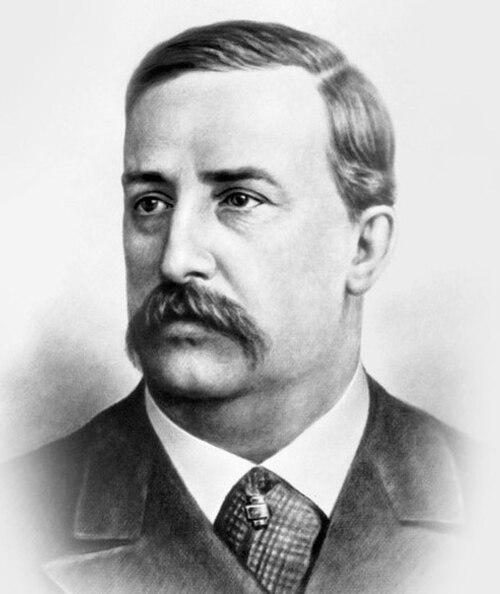
\includegraphics[width=\linewidth]{images/book3/borodin.jpg}
\end{minipage}\hspace{0.02\linewidth}%
\begin{minipage}[t]{0.18\linewidth}
\vspace{0pt}
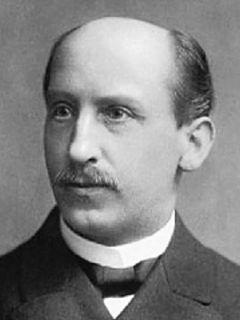
\includegraphics[width=\linewidth]{images/book3/claisen.jpg}
\end{minipage}\hfill
\begin{minipage}[t]{0.58\linewidth}
\vspace{0pt}
La reacción \omterm{def:b2:enolates-aldol:aldol}{aldólica} fue descrita en 1872 por Charles-Adolphe Wurtz y, de forma independiente, por Alexander
Borodin, químico de San Petersburgo más conocido hoy como compositor de \textit{El príncipe Ígor}.
Ludwig Claisen extendió las condensaciones de los compuestos carbonílicos a los ésteres en 1887. (Retratos: Borodin,
autor desconocido, dominio público; Claisen, por Veronica.villagrasa, CC BY-SA 4.0; Wikimedia Commons.)
\end{minipage}
\end{history}

\begin{safety}{\ghs[5mm]{GHS02}\,\ghs[5mm]{GHS05}\,\ghs[5mm]{GHS07}}
El etóxido de sodio y el diisopropilamiduro de litio son corrosivos y reaccionan con el agua; las disoluciones de LDA son
inflamables y se manipulan bajo gas inerte. El benzaldehído y la propanona son nocivos e inflamables.
% ledger: ghs:NaOEt, ghs:LDA, ghs:benzaldehyde, ghs:acetone
\end{safety}

\section{Ejercicios}

\begin{exercise}[$\star$]\label{exo:b2:enolates-aldol:1}
Dibújense los \omterm{def:b2:enolates-aldol:tautomerism}{tautómeros} enólicos de la butanona y de la ciclohexanona.
\end{exercise}

\begin{exercise}[$\star$]\label{exo:b2:enolates-aldol:2}
Ordénense por la acidez de su \ce{C-H} más ácido: propanona, pentano-2,4-diona, 3-oxobutanoato de etilo,
etano.
\end{exercise}

\begin{exercise}[$\star$]\label{exo:b2:enolates-aldol:3}
Dense el \omterm{def:b2:enolates-aldol:aldol}{aldol} y el producto de condensación del etanal con hidróxido de sodio.
\end{exercise}

\begin{exercise}[$\star$]\label{exo:b2:enolates-aldol:4}
Escríbase la \omterm{def:b2:enolates-aldol:decarboxylation}{síntesis malónica} del ácido hexanoico: ¿qué halogenoalcano se necesita?
\end{exercise}

\begin{exercise}[$\star\star$]\label{exo:b2:enolates-aldol:5}
Dibújense los \omterm{def:b2:enolates-aldol:kinetic-enolate}{enolatos cinético} y termodinámico de la 2-metilciclohexanona y las condiciones que dan
cada uno.
\end{exercise}

\begin{exercise}[$\star\star$]\label{exo:b2:enolates-aldol:6}
Dese el producto de la \omterm{def:b2:enolates-aldol:aldol}{condensación aldólica} cruzada del benzaldehído con la propanona (un equivalente
de cada uno) y explíquese por qué el benzaldehído no se condensa consigo mismo.
\end{exercise}

\begin{exercise}[$\star\star$]\label{exo:b2:enolates-aldol:7}
La hexano-2,5-diona en medio básico sufre una \omterm{def:b2:enolates-aldol:aldol}{condensación aldólica} intramolecular. ¿Qué anillo se forma? Explíquese la
elección entre los anillos posibles.
\end{exercise}

\begin{exercise}[$\star\star$]\label{exo:b2:enolates-aldol:8}
Escríbase la \omterm{def:b2:enolates-aldol:claisen}{condensación de Claisen} del etanoato de etilo y su producto tras el tratamiento ácido.
\end{exercise}

\begin{exercise}[$\star\star$]\label{exo:b2:enolates-aldol:9}
¿Cuáles de estos compuestos dan positivo el ensayo del yodoformo: propanona, pentan-3-ona, etanal, acetofenona?
\end{exercise}

\begin{exercise}[$\star\star\star$]\label{exo:b2:enolates-aldol:10}
Escríbase la ciclación de Dieckmann del hexanodioato de dietilo e indíquese el tamaño del anillo del producto.
\end{exercise}

\begin{exercise}[$\star\star\star$]\label{exo:b2:enolates-aldol:11}
La (\textit{R})-3-metilpentan-2-ona pierde su actividad óptica en hidróxido de sodio diluido, pero la
(\textit{R})-4-metilhexan-2-ona no. Explíquese.
\end{exercise}

\begin{exercise}[$\star\star\star$]\label{exo:b2:enolates-aldol:12}
Propóngase una vía hacia la 1,5-difenilpenta-1,4-dien-3-ona, y luego hacia una dienona con dos grupos arilo distintos,
y dígase por qué la segunda es más difícil.
\end{exercise}

\section{Problema: la dibencilidenacetona}

\begin{problem}[{Problema de fin de semana --- el enolato de la propanona y el papel del benzaldehído, las dos
condensaciones aldólicas, el producto conjugado, y la estequiometría y el rendimiento de una preparación}]
\label{pb:b2:enolates-aldol:1}
Preparación (datos de ejercicio): se agitan \qty{2.1}{mL} de benzaldehído y \qty{0.75}{mL} de propanona
en etanol con hidróxido de sodio acuoso; se separan cristales amarillos de 1,5-difenilpenta-1,4-dien-3-ona
(dibencilidenacetona); rendimiento del 75~\%. Densidades (\unit{g/cm^3}): benzaldehído 1.045, propanona 0.7845.
Masas molares (\unit{g/mol}): C 12.011, H 1.008, O 15.999.
% ledger: rho:benzaldehyde, rho:acetone, aw:C, aw:H, aw:O, ghs:dibenzalacetone

\medskip
\noindent\textbf{Parte I --- Los compañeros.}
\begin{enumerate}
  \item ¿Qué compañero tiene hidrógenos $\alpha$? ¿Cuántos?
  \item Dibújese el \omterm{def:b2:enolates-aldol:enolate}{enolato} de la propanona.
  \item ¿Por qué no puede formar un \omterm{def:b2:enolates-aldol:enolate}{enolato} el benzaldehído?
  \item ¿Por qué reacciona la propanona con el benzaldehído y no consigo misma?
  \item ¿Por qué un aldehído es mejor electrófilo que una cetona?
  \item ¿Por qué basta aquí el hidróxido como base?
\end{enumerate}

\medskip
\noindent\textbf{Parte II --- El mecanismo.}
\begin{enumerate}[resume]
  \item Escríbase la adición del \omterm{def:b2:enolates-aldol:enolate}{enolato} al benzaldehído.
  \item Escríbase la deshidratación del \omterm{def:b2:enolates-aldol:aldol}{aldol} formado.
  \item ¿Por qué es fácil aquí la deshidratación?
  \item ¿Por qué puede producirse la reacción una segunda vez?
  \item Escríbase la ecuación global.
  \item ¿Qué lleva la reacción hasta el final en esta preparación?
\end{enumerate}

\medskip
\noindent\textbf{Parte III --- El producto.}
\begin{enumerate}[resume]
  \item ¿Cuántos dobles enlaces \ce{C=C} tiene la dibencilidenacetona, y de qué configuración (principalmente)?
  \item ¿Por qué está favorecido el isómero (\textit{E},\textit{E})?
  \item Cuéntense los enlaces $\pi$ conjugados.
  \item ¿Por qué el compuesto es amarillo mientras que sus compañeros son incoloros?
  \item ¿Es quiral la dibencilidenacetona?
\end{enumerate}

\medskip
\noindent\textbf{Parte IV --- Estequiometría y rendimiento.}
\begin{enumerate}[resume]
  \item Calcúlense las masas molares del benzaldehído, la propanona y la dibencilidenacetona.
  \item Calcúlense las cantidades de los dos reactivos.
  \item ¿Qué reactivo es el limitante?
  \item Calcúlese la masa teórica de producto.
  \item ¿Por qué es preferible un ligero exceso de benzaldehído a un exceso de propanona?
  \item ¿Qué daría un exceso de propanona?
  \item Indíquese la masa de dibencilidenacetona obtenida con un rendimiento del 75~\%.
\end{enumerate}
\end{problem}
